\newpage
\subsubsection{Caso d'uso UC 4.3: Condivisione di una bolla lista-spesa.}
\label{Caso d'uso UC 4.3: Condivisione di una bolla lista-spesa.}
\begin{figure}[ht]
	\centering
	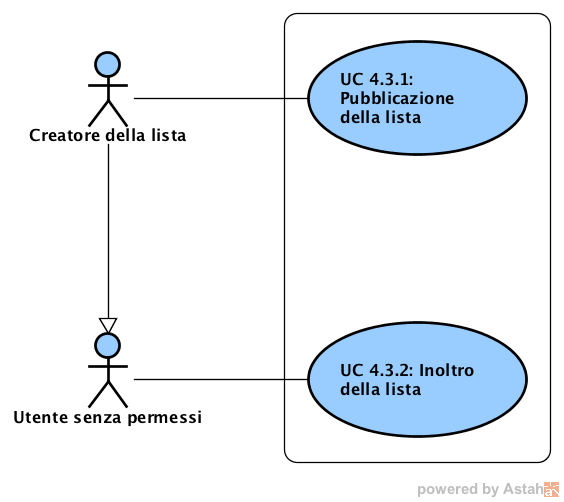
\includegraphics[scale=0.60]{Usecases/img/UC4.3.png}
	\caption{Caso d'uso UC 4.3: Condivisione di una bolla lista-spesa.}
\end{figure}

\FloatBarrier
\begin{itemize}
\item \textbf{Attori:} Creatore della lista.
\item \textbf{Descrizione:} Il Creatore della lista vuole condividere la bolla lista-spesa creata e può farlo in due modi:
\begin{itemize}
\item{Pubblicando la lista e ciò permetterà ai destinatari di interagire con essa.}
\item{Inoltrando la lista come messaggio normale. Ciò permetterà solo di visualizzarla in formato testuale senza poter, in alcun modo, interagire con essa.}
\end{itemize}
\item \textbf{Precondizione:} Il Creatore della lista vuole condividere la bolla lista-spesa creata. 
\item \textbf{Postcondizione:} Il Creatore della lista ha condiviso la bolla lista-spesa creata.
\item \textbf{Scenario principale:}
	\begin{itemize}
	\item{Pubblicazione della lista (UC 4.3.1).}
	\item{Inoltro della lista (UC 4.3.2).}
	\end{itemize}
\end{itemize}